\section{Inertial Confinement Fusion}
\label{sec:ICF}

	Traditionally, fusion power approaches aim to create plasma conditions hot enough to allow nuclear fusion and then maintain these conditions long enough (ideally indefinitely) to get a sufficient amount of power out. In these schemes, additional fuel is added to the system as fuel burns away without ever transitioning away from the desired plasma conditions. 
	
	Another approach is a pulsed scheme, one where a single component of fuel is brought to the desired temperature and density until all or most of it burns away. Instead of maintaining extreme plasma conditions, they would be recreated each time for each individual component of fuel. This process would be repeated at some frequency in order to achieve some desired power output.
	
	One immediate problem with this approach is the limited energy gain available. As we've seen from Figure \ref{fig:reactivities}, nuclear fusion requires temperatures of order 10 to 20 keV and the total energy received (for DT) is 17.6 MeV. Assume we expend some energy to create a DT plasma with $n_D=n_T=n/2$ and we burn some fraction $f$ of the fuel. The fractional energy gain $G$ would be:
	%
	\begin{equation}
		G = \frac{E_{gain}}{E_{spent}} = \frac{fnQ}{3/2\left(n_DT + n_TT\right)} = \frac{Qf}{3T}
	\end{equation}
	%
	In the absolute best case scenario $f=100\%$ and taking $T=20$ keV, we achieve a gain of roughly 600. This may seem like a lot, but it's extremely limiting from an engineering standpoint as it represents the absolute best we can possibly do. Once you start to consider any realistic inefficiencies (40\% from Carnot, 10\% from the heating process, 50\% fuel utilization, etc) the potential energy profit starts to diminish rapidly. This approach of heating the entire fuel volume is often referred to as \emph{volume ignition}.
	
	To get around this, we consider a hybrid approach that we'll refer to as \emph{hot-spot ignition} in the center. In this pulsed power approach, we will still only interact with a single fuel component at a time but we'll only heat some fraction of it to fusion conditions. The remaining \emph{cold fuel} will be heated from the fusion power itself; specifically from the charged particle products. For DT fusion, this means that the $\alpha$ particles (which only carry 20\% of the energy) will heat the remaining cold fuel. This creates a runaway process in the form of a propagating burn wave throughout the entire fuel volume. See Figure \ref{fig:hotspot} for a diagram of this idea.
	
	\begin{figure}[h!]
		\centering
		\caption{\todo{Hot spot}}
		\label{fig:hotspot}
	\end{figure}

	We only need the hot-spot to generate enough energy to heat up the cold fuel immediately around it. A detailed calculate of this is not entirely straightforward but let's say a factor of 2 more energy than what is required to heat it. Accounting for the fact that $\alpha$s only carry 20\% of the energy means we need a hot-spot $G$ of about 10. This means we need to burn about $f_{HS}=3\%$. 
	
	Let's consider now, how long it will take to burn away this fraction of fuel. Taking equation \ref{eq:reactionRateThermal} we can write down the differential equation that governs rate of fuel burn:
	%
	\begin{equation}
		\dfrac{dn}{dt} = - \frac{n^2}{2}\left<\sigma v\right>_{DT}
	\end{equation}
	%
	Or in terms of $f$:
	%
	\begin{equation}
		\frac{df}{dt} = (1-f)^2\frac{n_0}{2}\left<\sigma v\right>_{DT}
	\end{equation}
	%
	where $n_0$ is the initial fill density of the fuel. If we assume $\left<\sigma v\right>$ is roughly constant over the burn, we can solve for $f$ to get:
	%
	\begin{equation}
		f = \frac{n_0\left<\sigma v\right>_{DT}\tau}{2 + n_0\left<\sigma v\right>_{DT} \tau}
		\label{eq:fuelFraction}
	\end{equation}
	%
	Where $\tau$ is the duration over which the fuel is able to burn. 
	
	As a side note, this equation is important because it highlights the three key components involved in burning fusion fuel; density ($n_0$), temperature ($\left<\sigma v\right>$), and confinement time $(\tau)$. It is similar to (but not the same as) the Lawson criteria in this way. All approaches to fusion must raise some combination of these three factors high enough in order to efficiently produce fusion power. Often the difference between approaches come down to what factor is being focused.

	For inertial confinement fusion (ICF), we seek to minimize the complications associated with confining these extreme condition plasmas. We do this by recognizing that any plasma will take a finite amount of time to disassemble itself. If we can get the plasma to a final state that burns sufficiently fast, that finite amount of time will be sufficient. We have yet to discuss how we'll get the plasma to this state, but let's explore the requirements associated with trying to do that.
	
	Without any confinement, a plasma will disassemble at a rate proportional to the acoustic ion sound speed:
	%
	\begin{equation}
		c_s = \sqrt{\frac{4T}{m_{DT}}}
	\end{equation}
	%
	Here we have assumed the electrons have the same temperature ($T_e$) as the ions. The fuel will continue burning so long as the density of the fuel has not sufficiently changed. Let's assume our fuel is all contained is a sphere of radius $R$ such that we can allow it to disassemble for some $\tau< R/c_s$ before the burn is too negatively effected. The exact value for $\tau$ is a bit arbitrary, and deserves detailed calculations, but most literature takes it to be $R/4c_s$. We can plug this into equation \ref{eq:fuelFraction} to show:
	%
	\begin{equation}
		\begin{split}
			f &= \frac{n_0\left<\sigma v\right>_{DT} R / 4c_s}{2 + n_0\left<\sigma v\right>_{DT} R / 4c_s} \\
			& = \frac{n_0m_{DT}R}{n_0m_{DT}R + \frac{8 c_s m_{DT}}{\left<\sigma v\right>_{DT}}}\\
			&= \frac{\rho R}{\rho R + H_B}
		\end{split}
		\label{eq:burnFraction}
	\end{equation}
	%
	Here we've defined a few new terms. $\rho R$ is the areal density of the plasma and $H_B$ is the so called \emph{burn parameter} which depends entirely on $T$. By defining our $\tau$ though the ICF approach, we have reduced our parameter space from three to two parameters. This means we can easily plot the fusion requirements for ICF schemes. 
	
		\begin{figure}[h!]
		\centering
		\includegraphics[scale=0.7]{fusionRequirements}
		\caption[ICF Fusion Requirements]{Areal density and temperature requirements to burn certain fuel fractions in ICF schemes. Dashed curves correspond to the hot-spot requirement of $f_{HS}=3\%$ and solid curves correspond to a cold-fuel high gain requirement of $f=30\%$. Different fuels are plotted as different colors. DT, D3He, DD, and p11B are plotted as red, blue, green, and yellow respectively.  }
		\label{fig:fusionRequirements}
	\end{figure}

	Using Figure \ref{fig:fusionRequirements} we can set some requirements for an ICF approach to achieve high gain. First we have the hot-spot ignition requirement from before of $f_{HS}=3\%$ which corresponds to an areal density of roughly 0.3 g/cm$^2$ at temperatures around 20 keV. For the rest of the fuel assembly, we want burn fractions high enough to produce substantial gain, but low enough to minimize the areal density requirement. For now let's take $f=30\%$ which corresponds to areal densities around 4-5 g/cm$^2$ for DT fuels. 
	
	The next question to address is how to get these areal densities. The most naive way would be to construct a fuel assembly with $R$ sufficiently large so as to meet the requirement. If we take the density of DT ice to be roughly 0.225 g/cm$^3$ we can achieve a $\rho R$ of 4.5 g/cm$^2$ with an $R=20$ cm. We can calculate the total energy released from this assembly:
	%
	\begin{equation}
		\begin{split}
			E_{tot} & \sim \mathcal{R}_{12} \times \tau \times V \times f \times Q \\
			& \sim \left(n_Dn_T\left<\sigma v\right>_{DT}\right) \times \left( \frac{R}{4 c_s}\right) \times \left(\frac{4}{3} \pi R^3\right) \times \left(\frac{\rho R}{\rho R + H_B}\right) \times Q \\
			& \sim \frac{\pi \left<\sigma v\right>_{DT}}{3 m_{DT}^2 c_s} \left(\frac{\rho R}{\rho R + H_B}\right)Q \left(\rho R\right)^2 R^2
		\end{split}
		\label{eq:littleboyyield}
	\end{equation} 
	%
	Plugging in our numbers get us $E_{tot} \sim 5 \times 10^{14}$ J or roughly 12 kT of TNT. Roughly the yield from the Little Boy bomb dropped Hiroshima in 1945. While this is certainly an impressive yield of energy, it's not particularly conducive to our goal of designing a fusion reactor that doesn't detonate itself and the people around it. In order to ensure our reactor is safe and reasonable, we must put an additional constraint on $E_{tot}$. However, the only free parameter left in equation \ref{eq:littleboyyield} is $R$. Rearranging the equation we get:
	%
	\begin{equation}
		R = \frac{1}{\rho R} \sqrt{\left(\frac{3 m_{DT}^2 c_s}{\pi \left<\sigma v\right>_{DT}}\right) \left(\frac{\rho R + H_B}{\rho R}\right)\left(\frac{E_{tot}}{Q}\right) }
	\end{equation}
	%
	It's debatable what limit we can set for $E_{tot}$, but most sources seem to be of the order 100 MJ. Plugging in our numbers gets us a $R$ of roughly 280 $\mu$m which makes the corresponding $\rho = 160$ g/cm$^2$, which is roughly 700 times the solid density of the DT ice.  So, in order to achieve reasonably low fusion energies (while still getting high gain) using an ICF scheme requires compressing DT fuel to extreme densities. In reality, the hot-spot generally starts as DT vapor for a variety of reasons and thus requires much more compression to reach it's target areal density of 0.3 g/cm$^2$. Ignition designs generally quote convergence ratios (the ratio between the initial and final radii) of 20-35. 
	
	\todo{Currently no discussion on shocks / how ignition temperature is achieved} \\
	
	There are a handful of methods that can be used to achieve this compression, but all major methods today use high power lasers. The basic idea is to start with a small hallow spherical target of DT ice surrounded by an ablator material. Various ablators have been considered including plastic, beryllium, and high-density carbon (diamond or HDC). The ablator material is rapidly and symmetrically heated by the laser causing it to expand outward and force the rest of the target inwards. This kind of \emph{direct drive} of the target is the major approach being explored at the OMEGA laser Facility discussed in Section \ref{sec:OMEGA}. 
	
	\begin{figure}[h!]
		\centering
		\caption{\todo{ICF Direct Drive}}
	\end{figure}
	
	One of the hardest challenges of ICF is the symmetric compression of the fuel. Any asymmetries get severely amplified during the compression and risk tearing the fuel assembly apart before peak compression is reached. An alternative drive technique called \emph{indirect drive} tries to improve symmetry by first heating the inside of a can referred to as a \emph{hohlraum}. The hohlraum is made of a high Z material like gold or depleted-uranium and emits black-body radiation once it's heated. The x-rays from this emission then go on to heat the ablator which achieves compresion exactly as described before. This approach to ICF is the main approach being explored at the Nation Ignition Facility (NIF) discussed in Section \ref{sec:NIF}. 
	
	\begin{figure}[h!]
		\centering
		\caption{\todo{ICF Indirect Drive}}
	\end{figure}

	

